\section{Alternativa regulatorstrukturer}

\paragraph{Kaskadreglering}
Ideen bakom kaskadreglering är att försöka reglera ett system med hjälp av en mellanliggande signal. Detta beskrivs av blockschemat i figur \ref{fig:cascade_control}.
\begin{figure}[!ht]
	\centering
	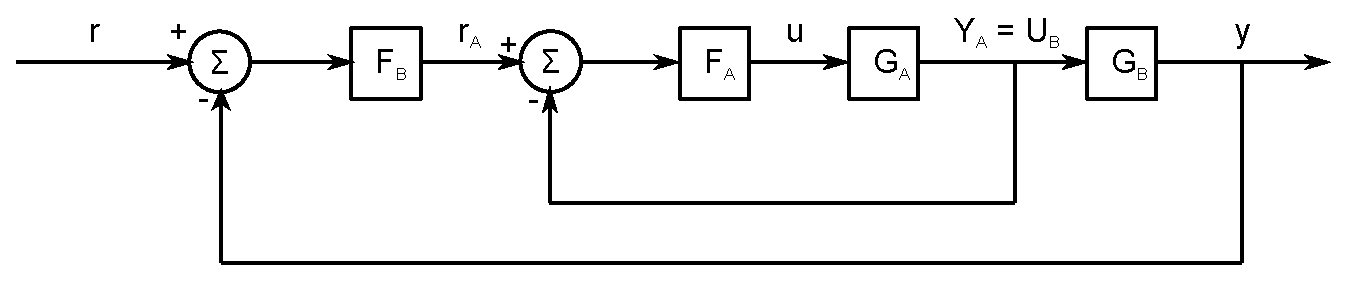
\includegraphics[width = 0.8\textwidth]{./Images/cascade_control.eps}
	\caption{Blockschema av kaskadreglering.}
	\label{fig:cascade_control}
\end{figure}
Kretsen i mitten reglerar mellansignalen $u$ mot ett visst värde $U_{B}$. Detta är värdet som regulatorn $F_{B}$ vill ha. Om detta skall fungera, måste den inre regleringen vara snabbare än den yttre.

\paragraph{Framkoppling}
Ideen bak framkoppling är att försöka reglera bort en mätbar störsignal. Detta visas i blockschemat i figur \ref{fig:forward_connection}.
\begin{figure}[!ht]
	\centering
	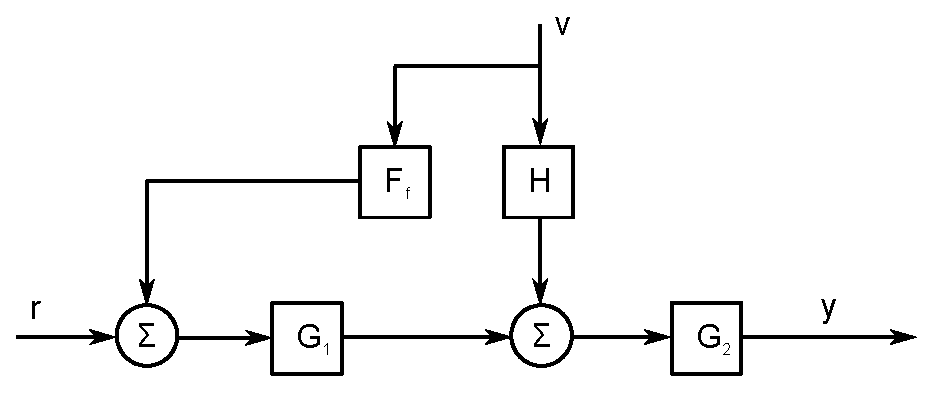
\includegraphics[width = 0.6\textwidth]{./Images/forward_connection.eps}
	\caption{Blockschema av framkoppling.}
	\label{fig:forward_connection}
\end{figure}
Vi önskar nu välja $F_{f}$ så att störsignalen ej har någon inverkan.

Vi har
\begin{align*}
	Y = G_{2}(HV + G_{1}(R + F_{f}H)) = G_{2}((H + G_{1}F_{f})V + G_{1}R).
\end{align*}
Därmed kommer $V$-termen försvinna om vi väljer
\begin{align*}
	F_{f} = -\frac{H}{G_{1}}.
\end{align*}

En fördel med detta är att man kan reglera sitt system innan störningen får en inverkan. Det kan dock uppstå problem med att man får rena deriveringstermer, men dessa kan lösas genom att approximera $F_{f}$ nära $s = 0$.

\paragraph{Otto Smith-regulatorn}
Syftet med Otto Smith-regulatorn är att reglera system med tidsfördröjning. Fasfördröjningen från en sån ökar med $\omega$, vilket gör det svårt att reglera.

För att reglera detta, bestäm först ett $F$ så att ditt äntliga system (till exempel det slutna reglersystemet) får bra egenskaper om man ignorerar tidsfördröjningen. Om reglering av det icke-fördröjda öppna systemet $G$ ger en regulator $F$, inför nu regulatorn
\begin{align*}
	F' = \frac{F}{1 +(1 - e^{-sT})FG},
\end{align*}
där $T$ är systemets fördröjning. Detta kommer ge
\begin{align*}
	G_{\text{c}} = \frac{FG}{1 + FG}e^{-sT}.
\end{align*}

\paragraph{Internal Model Control}
Ideen bak IMC illustreras i figur \ref{fig:imc}.
\begin{figure}
	\centering
	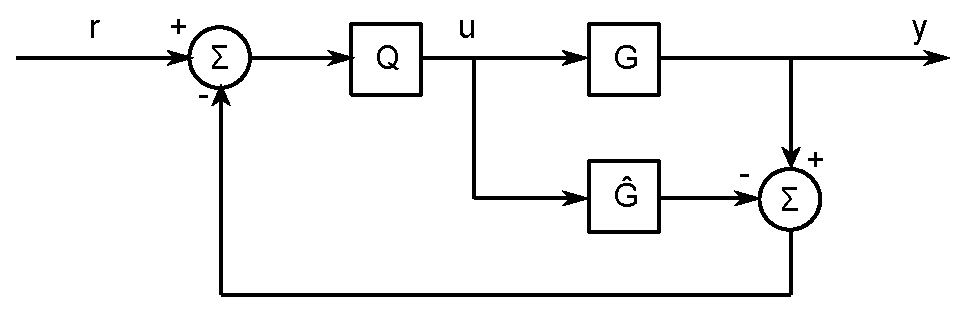
\includegraphics[width = 0.6\textwidth]{./Images/imc.eps}
	\caption{Blockschema av IMC.}
	\label{fig:imc}
\end{figure}
Vi har här introducerat $\hat{G}$ som vår modell av systemet.

Flödesschemat ger
\begin{align*}
	U = \frac{Q}{1 - Q\hat{G}}(R - Y).
\end{align*}
Om vi jämför detta med standardvarianten $U = F(R - Y)$, ser vi att
\begin{align*}
	F = \frac{Q}{1 - Q\hat{G}}.
\end{align*}
Detta betyder att alla problem vi har studerat kan omformuleras som ett IMC-problem.

Varför inför vi detta? Först av allt kan vi på något sätt hitta alla regulatorer som stabiliserar systemet genom att titta på stabila $Q$, vad nu det betyder. Vidare är det enkelt att studera det slutna systemet, ty om vi har en perfekt modell, försvinner återkopplingen, och $Y = GQR$. Detta är linjärt i $Q$, medan fall vi har studerat tidigare inte har varit linjära i $F$.

Betrakta specialfallet där vi vil ha $Y = HR$. Då väljer vi $Q = \frac{H}{G}$. Detta ger
\begin{align*}
	F = \frac{1}{G}\frac{H}{1 - H},
\end{align*}
som är resultatet vi känner från tidigare. På liknande sätt kan andra reglerproblem formuleras med IMC.